%BILD
\subsection{Model-View-ViewModel}
Durch die Entwicklung des Windows Presentation Foundation Framework (WPF) durch Microsoft entstand 2005 das Architekturmodell \ac{MVVM}, das ein fester Bestandteil von Silverlight\footnote{Silverlight is a cross-browser, cross-platform plug-in for delivering media and rich interactive applications for the Web} ist. Ebenso werden existierende Frameworks um \ac{MVVM} erweitert\cite{Jaeckle2015}.

\begin{figure}[h] 
\centering
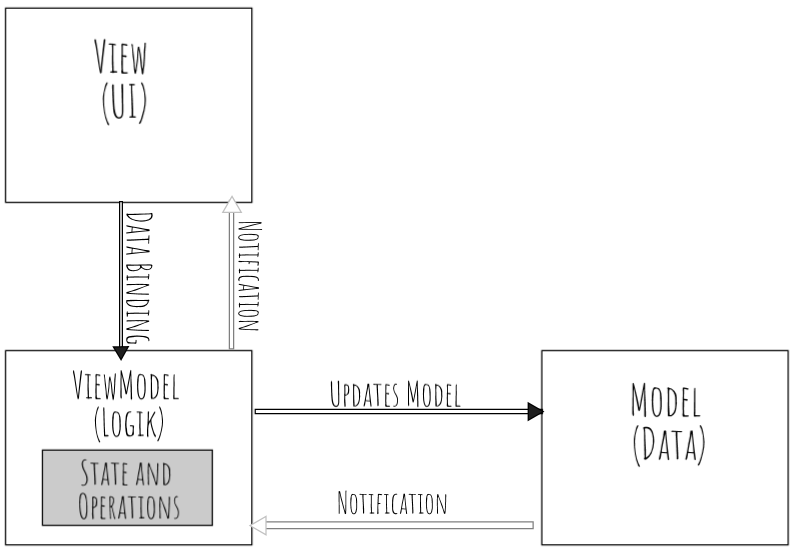
\includegraphics[scale=0.45]{fig/mvvmv2.png} 
\caption{Komponente des MVVM Architekturmusters}
\label{fig:MVVM}
\end{figure} 
Wie die drei Komponente View, ViewModel und Models miteinanderer zusammenh\"angen und kommunizieren, wird im folgenden erl\"autert und durch Abbildung \ref{fig:MVVM} abgebildet.

\subsection*{Data-Binding}
Wie schon davor erw\"ahnt wurde, kennt die View das ViewModel und das ViewModel kennt das Model, jedoch nicht vice versa, was die Pfeile in Abbildung \ref{fig:MVVM} illustriert.
Damit die View mit dem ViewModel interagieren kann, wird in WPF ein sogenanntes Data-Binding verwendet.
Durch die Datenbindung wird eine Verbindung zwischen der View (User Interface (UI)) und dem ViewModel (Logik) hergestellt. Wenn das Model (Daten) die korrekten Benachrichtigung bereitstellt, k\"onnen die eingebundenen Daten automatisch die \"Anderung des Wertes annehmen und in der View wiedergeben\cite{Cai2017}.
Eine Verbindung besteht zumeist aus vier Komponenten: ein Zielobjekt, eine Zieleigenschaft, die eine Abh\"angigkeitseigenschaft sein muss, eine Quelle und ein Pfad zum Wert, das verwendet wird. 
Wenn eine Verbindung aufgebaut ist, ist die Richtung des Datenflusses entscheidend und wichtig. Hier gibt es drei verschiedene Wege die Daten zu senden bzw. zu empfangen.
\begin{itemize}
\item One-Way Bindung
\item Two-Way Bindung
\item One-Way To Source Bindung
\end{itemize}
\begin{figure}[h] 
\centering
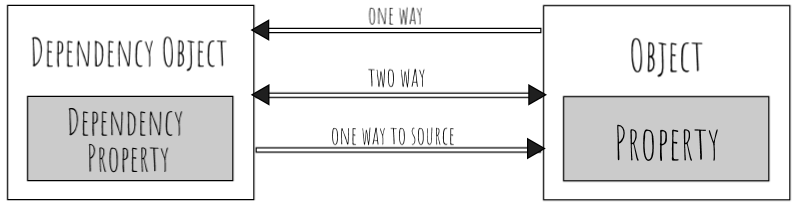
\includegraphics[scale=0.55]{fig/Data-Binding.png} 
\caption{Datenbindung zwischen View und ViewModel}
\label{fig:DataBinding}
\end{figure} 
Die View, das Bindungsziel, besitzt ein Dependency(engl. f\"ur abh\"angig) Objekt mit einer Dependency Property, einer Eigenschaft, wie zum Beispiel einem String. Diese sind abh\"angig voneinander. Das ViewModel, die Bindungsquelle, besitzt ein Objekt mit einer Property. Eine One Way Bindung l\"asst \"Anderungen an der Quelle zu und aktualisiert die Zieleigenschaften automatisch. Diese Verbindung ist vor allem n\"utzlich, wenn schreibgesch\"utzte Elemente in der UI vorhanden sind, denn \"Anderungen an den Zieleigenschaften sind bei einer One Way Bindung nicht m\"oglich.
Eine Two Way Bindung erm\"oglicht dem User, \"Anderungen vorzunehmen. Hierbei werden die Zieleigenschaften ver\"andert und automatisch die Quelleigenschaften aktualisiert. Andersherum geschieht genau das gleiche, analog zur One Way Bindung. F\"ur zum Beispiel zu bearbeitende Formulare oder andere interaktive Situatuionen, die vermutlich Abh\"angigkeitseigenschaften aufweisen, ist diese Bindung r\"atlich.
Die kontr\"are Bindung zur One Way Bindung ist die One Way To Source Bidnung, diese aktualisiert automatisch die Quelleigenschaften wenn die Zieleigenschaft ge\"andert wurde.
\subsection*{Notifications}
Um die \"Anderung zu erkennen, muss die Quelle einen Benachrichtgungsmechanismus beinhalten. In der Regel ist dies die \texttt{INotifyPropertyChanged} Implementierung. Bei dieser Implementierung wird ein Objekt an die UI gebunden, das das Ereignis \texttt{PropertyChanged} enth\"alt und dies ausl\"ost, sobald eine \"Anderungen an der Eigenschaft des Objektes wahrgenommen wird. Diese \"Anderung wird von dem Model an das ViewModel gesendet, das dann die Aktualisierung an der Quelleigenschaft vornehmen kann und die \"Anderung in der View angezeigt.
Die Quellaktualisierungen werden anhand \texttt{UpdateSourceTrigger}, die Eigenschaften enthalten, die bestimmen, wann und warum die Benachrichtigung ausgel\"ost wird,  ausgel\"ost. 


\subsection*{Fazit}
Das Ziel des Architekturmuster ist, wie auch bei dem Architekturmuster \ac{MVC}, das der Vorreiter von \ac{MVVM} ist, das Trennen der Logik und der Pr\"asentations Schicht bzw. der View.
Die Vorteile des Entwurfsmuster \ac{MVVM} sind:
\begin{itemize}
\item Durch die Trennung m\"ussen \"Anderungen, die an dem Model vorgenommen werden, nicht an der View ge\"andert werden\cite{tutorialspointMVVM} .
\item W\"ahrend der Entwicklung k\"onnen die Entwickler und die Designer unabh\"angig voneinander an den Komponenten arbeiten\cite{Pete2016}.
\item Modultests f\"ur das ViewModel und das Model k\"onnen ohne die View erstellt werden\cite{Pete2016}.
\item Die View kann beliebig ausgetauscht und wiederbenutzt werden, da die View unabh\"angig von den anderen Komponenten ist\cite{Pete2016}.
\item Die Weiterentwicklung sowie die Instandhaltung kann durch die Trennung detaillierter vorgenommen werden, ohne dass die  \"Anderungen negative Auswirkungen auf das System haben\cite{tutorialspointMVVM}.
\end{itemize}
Die Nachteile des Architekturmuster sind in der Minderheit.
F\"ur viele Entwickler ist \ac{MVVM} f\"ur einfache Oberfl\"achen zu m\"achtig und ebenso f\"ur gr\"o\ss{}ere F\"alle kann es schwierig sein, das ViewModel zu konstruieren.
Wenn die Datenbindung komplexer ist, wird das Debugging ebenso problematischer\cite{tutorialspointMVVM}.

